\documentclass[a4paper,11pt, twocolumn]{article}
\usepackage[rightcaption]{sidecap}
\usepackage[font={scriptsize,it}]{caption}
\usepackage{graphicx}
\usepackage{amsmath}
\usepackage{amssymb}
\usepackage{subcaption}

% define the title
\author{Alun Meredith}
\title{Maching Learning - 2}

\begin{document}
% generates the title
\maketitle

\section{Distance from a point to a line}

The general equation for a straight line in two dimensions is $a_0 + a_1x_1 + a_2x_2 = 0$, or $\mathbf{ax}=0$ in vector notation, where $\mathbf{x_0}$ is a bias term. The gradient of this line is given by$ -\frac{a_1}{a_2} $ . Consider the perpendicular line to this which passes through the origin, $x_2 = \frac{a_2}{a_1}x_1$ and equating the two lines to get the point on the line closest to the origin $\frac{-a_0a_1}{a_1^2+a_2^2}, \frac{-a_0a_2}{a_1^2+a_2^2}$. Finally we calculate the distance to this point using Pythagoras' Theorem.
 
\begin{equation}
	d = \frac{a_0}{\sqrt{a_1^2+a_2^2}}
\end{equation} 

This result can be generalised to show the perpendicular distance from any point $P(m,n)$ and a line by considering a parallel line which passes through the point $P$ and comparing their distance to the origin (Figure \ref{fig:diagram1}): \footnote{//www.intmath.com/plane-analytic-geometry/perpendicular-distance-point-line.php} 

\begin{equation}
d = \frac{|a_0+a_1m+a_2n|}{\sqrt{a_1^2+a_2^2}}
\end{equation}  

\begin{SCfigure}[0.4][ht]
\caption{Geometric description of distance from a point to a line}
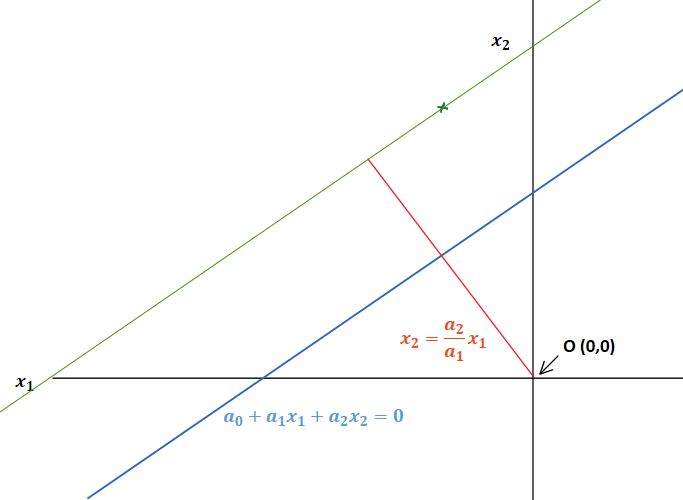
\includegraphics[width=0.25\textwidth]{diagram2.jpg}
\label{fig:diagram1}
\end{SCfigure}

\section{Bayes' Linear Classifier}

We are interested in classifying data through a linear decision boundary. To do this two sample distributions were taken from a Gaussian population distribution and transformed as shown in lab one so that their means where equal to $m_1^{(1)}=[0, 2]$ and $m_2^{(1)}=[1.5, 0]$ respectively and their covariances were equal. 
$C = \begin{bmatrix}
2 & 1 \\
1 & 2
\end{bmatrix} $

These distributions overlap significantly (figure \ref{fig:fig3a}). Two non-overlapping distributions, with the same covariance C, were produced for comparison. $m_1^{(2)} = [4,0]$ and $m_2^{(2)} = [0,4]$ (fig \ref{fig:fig3}). 

Given this training data we want to be able to classify any new observation with given features $x_1, x_2$ to the distribution it belongs to $P[\omega_j|\mathbf{x}]$. Bayes' theorem (\ref{equation:bayes}) gives a useful tool for assessing this:

\begin{equation}
P[\omega_j|\mathbf{x} = \frac{p(\mathbf{x}|w_j) P[\omega_j]}{\sum_{k=1}^n p(\mathbf{x}|w_i) P[\omega_i]}
\label{equation:bayes}
\end{equation}

To calculate this we need to know the prevalence (prior) $P[\omega_i]$ and the likelihood $\mathbf{x}|w_i)$. The prevlance for this case is simply $\frac{1}{2}$ because neither distribution is inherently more likely in the population. The likelihood is the probability density of each distribution at a point $P$. This is usually estimated from the training data. However for this example we know the population distribution (from which we sampled) so we don't have to make an estimate:

\begin{equation}
\label{equation:gaussian}
\scriptstyle
\frac{1}{(2\pi)^{p/2}(det(C))^{\frac{1}{2}}}exp\left\lbrace-\frac{1}{2}(\mathbf{x-m_1})^t\mathbf{C}^{-1}(\mathbf{x-m_1})\right\rbrace
\end{equation}

To evaluate which distribution is more likely, $p[\omega_1|x] \lessgtr p[\omega_2|x]$ using Bayes' theorem we find the boundary where they are equal. By substituting the population distributions (\ref{equation:gaussian}) into Bayes theorem (\ref{equation:bayes}) and simplifying like terms we get the linear classifier below.

\begin{align}
&\mathbf{w^tx} + b \lessgtr 0 \nonumber \\
&\mathbf{w} = 2\mathbf{C^{-1}(m_2 - m_1)}  \\
&b = \mathbf{(m_1^tm_1 - m_2^tm_2)} - log\{\frac{P[\omega_1]}{P[\omega_2]\}} \nonumber
\end{align}
In this case the priors are equal so that term is equal to 0. The linear classifiers for both our overlapping and separate cases are shown on figure \ref{fig:fig3}.

\begin{figure}[b]
\centering
\begin{subfigure}{.22\textwidth}
	\centering
	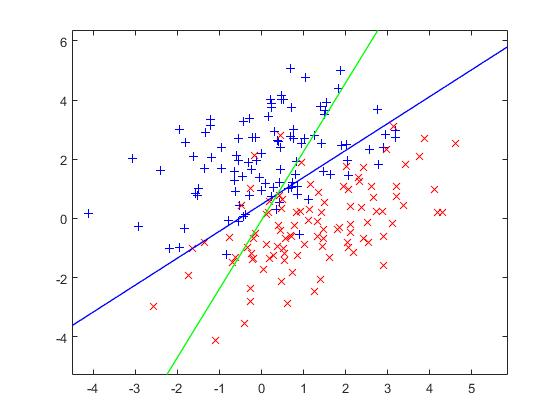
\includegraphics[width=\textwidth]{perceptron4.jpg}
	\subcaption{Overlapping distributions $\omega_i^{1}$}
	\label{fig:fig3a}
\end{subfigure}
\begin{subfigure}{.22\textwidth}
	\centering
	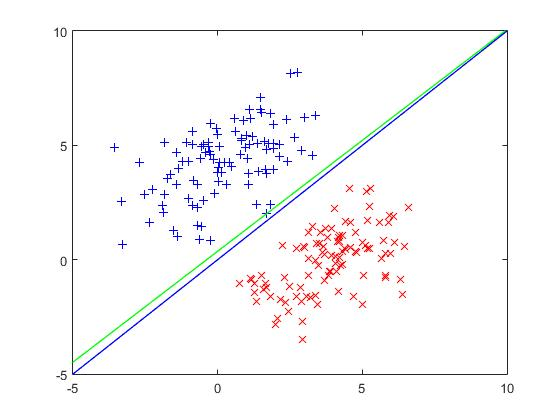
\includegraphics[width=\textwidth]{perceptron3.jpg}
	\subcaption{Distinct distributions $\omega_i^{2}$}
	\label{fig:fig3b}
\end{subfigure}
\caption{Blue line: Bayes' linear classifiers \\ Green line: Perceptron classifier (250,000 iterations)}
\label{fig:fig3}
\end{figure}

The classifiers perform quite well, accurately classifying all the observations in \ref{fig:fig3b} and leaving only a handful of misclassified observations in \ref{fig:fig3a}. Note it is impossible to classify all the observations correctly with a linear decision boundary.

These Bayesian classifiers assumed the data was both normally distributed and with equal covariance in order to formally work. While we are happy to do this because we know the population distribution precisely real world applications are not always this simple. However this naive simplification is often fairly accurate as long as you transform the data to approximate a normal distribution first. 
 
\section{Perceptron Algorithm}

Perceptron is an algorithm which produces a linear classifier. It randomly assigns the weights $a_0, a_1, a_2$ to produce a linear classification boundary, then iterates the weights by taking a random training set observation and if incorrectly classified shifts the weights towards that point. 

In the Bayes' linear classifier the boundary was produced from the population distribution, the perceptron algorithm uses the training examples. By looking at figure \ref{fig:fig3} we can see that after 250,000 iterations of the algorithm perceptron approximates the Bayes' classifier quite well, however for the overlapping distributions perceptron remains performs worse. 

By assessing how our algorithm performs against a test set over time we can evaluate what is happening (figure \ref{fig:fig4}). We can see that for the distinct populations perceptron reaches 100\% accuracy quickly, however the overlapping datasets shows a minima here which continues to oscillate noisily after that. This is because after the minima when perceptron sees a datapoint that it has still misclassified it tries to correct itself, depending on how extreme the outlier is the bigger changes it makes. 
\begin{figure}[ht]
\centering
\begin{subfigure}{.22\textwidth}
	\centering
	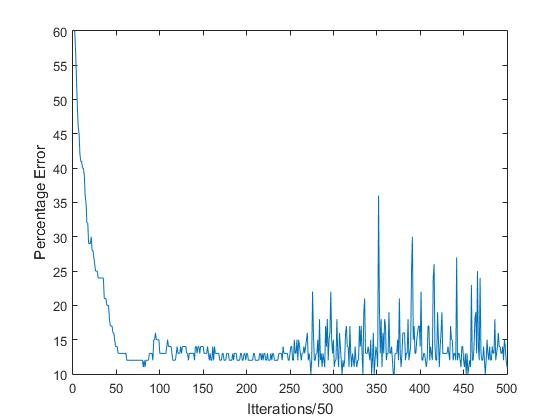
\includegraphics[width=\textwidth]{perceptron1.jpg}
	\caption{Overlapping distributions $\omega_i^{1}$}
	\label{fig:fig4a}
\end{subfigure}
\begin{subfigure}{.22\textwidth}
	\centering
	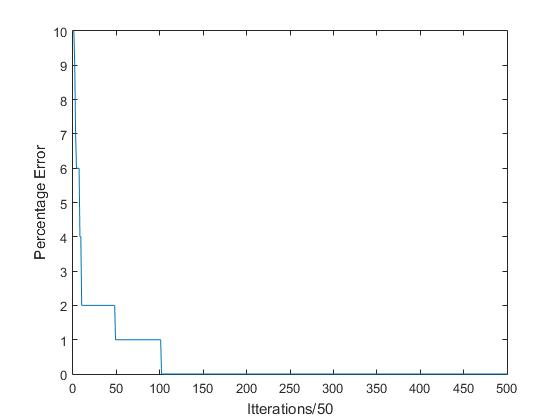
\includegraphics[width=\textwidth]{perceptron2.jpg}
	\caption{Distinct distributions $\omega_i^{2}$}
	\label{fig:fig4b}
\end{subfigure}
\caption{Accuracy over iterations of perceptron on test set}
\label{fig:fig4}
\end{figure}

\end{document}